In our scenario where occupants enter and exit the room constantly, typically within seconds or minutes of each other, it is somewhat difficult to find the immediate use of predicting an occupant's future actions. However, our partner team from Kenya expressed a need for such a system because they have had issues with thefts. Incorporating such a feature to their surveillance systems could warn a guard whenever suspicious activity might occur. A suspicious activity could involve a person moving too close to a given exit - possibly leading to a restricted area. In order to calculate a somewhat reliable prediction, we need to capture and store data about the behavior of previous occupants. When the data set grows, the prediction gradually becomes smarter and generally more precise. In order to satisfy the prediction requirement, various existing solutions have been considered, namely the \emph{k-nearest neighbors algorithm} and an existing prediction model, the hidden Markov model. The two solutions will be covered briefly. The former assigns a given object to a group depending on the \emph{k} nearest objects. To apply this to our scenario we imagined previously observed occupant positions being separated into groups dependent upon the chosen exit. Given any position we would analyze the \emph{k} neighboring previous positions of distinct occupants and predict the exit to be that of the majority.
\begin{figure}
\centering
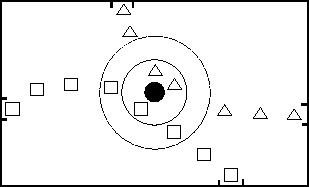
\includegraphics{prediction_figures/knn_room}
\caption{An illustration of the \emph{k-nearest neighbors algorithm}.}
\label{fig:knn}
\end{figure}
Figure~\ref{fig:knn} depicts an example where the center dot is the current position and the squares and triangles are previous occupant positions who chose separate exits. The circle with the solid line resembles a situation where \emph{k=3} which indicates that the occupant at the center is most likely to take the same exit as the occupants previously positioned at the triangle positions. The circle with the dashed line resembles a situation where \emph{k=5}. This yields a different output where the occupant is most likely to choose the same exit as the occupants previously residing at the positions of the squares. The approach has proven to be inefficient on larger data sets~\cite{bhatia}, which can be averted by performing clever data reduction. This, however, deemed the approach out of the scope of this project.
\begin{figure}
\centering
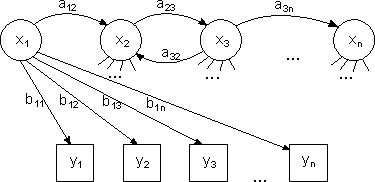
\includegraphics{prediction_figures/markov}
\caption{An illustration of the hidden Markov model.}
\label{fig:markov}
\end{figure}

Figure \ref{fig:markov} depicts the different parameters a hidden Markov model works with. Each \(x\) is a state and each \(y\) is a possible observation, where \(a\) is a state transition probability and \(b\) is an output probability. When translating this to our scenario we need to define what exactly a state and an observation is and how to calculate the different probabilities. Since the ultimate goal is to predict what exit an occupant is going to take, a possible observation could be that an occupant exits a room at a given location. A state could depict a room area where a transition to another room area would have a state transition probability \(a\). Given an occupant resides in any room area, \(b\) is the probability that the person will exit at a given location. Typically, the process is as follows; random probability values are assigned to \(a\) and \(b\) (maybe a ref to jahmm or something else). Gradually, these values are updated to reflect actual observed actions of occupants. Over time, the probabilities are modified and represent how the average occupant is moving given a current location, resulting in more accurate predictions - this process is commonly referred to as training. Even with the inclusion of a training procedure, the predictions will be incredibly unreliable in the beginning until a large enough data set has been collected. (DISCUSS, this might be wrong) Furthermore, imagine a scenario where an even number of occupants move from one exit to another in both directions, evenly split. At any location along the path the probabilities to each exit remain equal, since equally many previous occupants have taken each exit given the current location. In an attempt to partially avoid these issues, or at least produce some more reliable results with lesser data sets, we wanted to establish rule sets and integrate those into the calculations. Thus, we chose to design our own prediction model, heavily inspired by the hidden Markov model, since the original interpretation of states and probabilities as depicted in figure \ref{fig:markov} is maintained. The custom model is explained in detail in Section~\ref{ssub:designcustomprediction}. 

Figure \ref{fig:markov} depicts the different parameters a hidden Markov model works with. Each \(x\) is a state and each \(y\) is a possible observation, where \(a\) is a state transition probability and \(b\) is an output probability. When translating this to our scenario we need to define what exactly a state and an observation is and how to calculate the different probabilities. Since the ultimate goal is to predict what exit an occupant is going to take, a possible observation could be that an occupant exits a room at a given location. A state could depict a room area where a transition to another room area would have a state transition probability \(a\). Given an occupant resides in any room area, \(b\) is the probability that the person will exit at a given location. Typically, the process is as follows; random probability values are assigned to \(a\) and \(b\) (maybe a ref to jahmm or something else). Gradually, these values are updated to reflect actual observed actions of occupants. Over time, the probabilities are modified and represent how the average occupant is moving given a current location, resulting in more accurate predictions - this process is commonly referred to as training. Even with the inclusion of a training procedure, the predictions will be incredibly unreliable in the beginning until a large enough dataset has been collected. (DISCUSS, this might be wrong) Furthermore, imagine a scenario where an even number of occupants move from one exit to another in both directions, evenly split. At any location along the path the probabilities to each exit remain equal, since equally many previous occupants have taken each exit given the current location. In an attempt to partially avoid these issues, or at least produce some more reliable results with lesser data sets, we wanted to establish rule sets and integrate those into the calculations. Thus, we chose to design our own prediction model, heavily inspired by the hidden Markov model, since the original interpretation of states and probabilities as depicted in figure \ref{fig:markov} is maintained. The custom model is explained in detail in section \ref{ssub:designcustomprediction}.